\documentclass[11pt, a4paper]{article}

\usepackage{graphicx}
\usepackage[a4paper,top=3cm,bottom=2cm,left=2cm,right=2cm,marginparwidth=1.75cm]{geometry}
\usepackage[english]{babel}
\usepackage[utf8x]{inputenc}
\usepackage{subfig}
\usepackage{float}
\usepackage{amsmath}
\usepackage{amssymb}
\usepackage{mhchem}
\usepackage{hyperref}
\usepackage{tikz}
\usepackage{cancel}

\graphicspath{ {./images} }
\newcommand*{\qed}{\hfill\ensuremath{\quad\square}}%
\newcommand*{\rad}{\ensuremath{\,\text{rad}}}
\newcommand*{\R}{\ensuremath{\mathbb{R}}}
\newcommand*{\C}{\ensuremath{\mathbb{C}}}
\renewcommand*{\Re}{\operatorname{Re}}
\renewcommand*{\Im}{\operatorname{Im}}
\renewcommand*{\epsilon}{\varepsilon}
\renewcommand*{\phi}{\varphi}

\makeatletter
\renewcommand*\env@matrix[1][*\c@MaxMatrixCols c]{%
  \hskip -\arraycolsep
  \let\@ifnextchar\new@ifnextchar
  \array{#1}}
\makeatother

\newtheorem{theorem}{Theorem}

%------------------------------------------------
%Templates for images and figures
% \begin{figure}[h]
%   \centering
%   \subfloat[caption 1]{{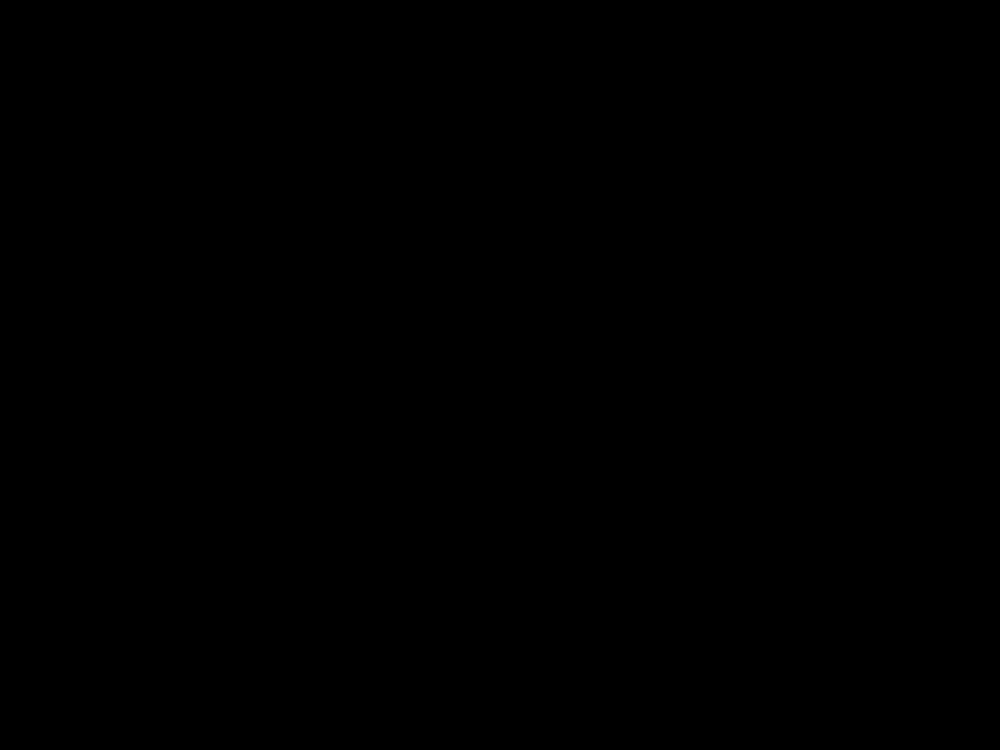
\includegraphics[width=30mm]{images/placeholder.png}}}%
%   \qquad
%   \subfloat[caption 2]{{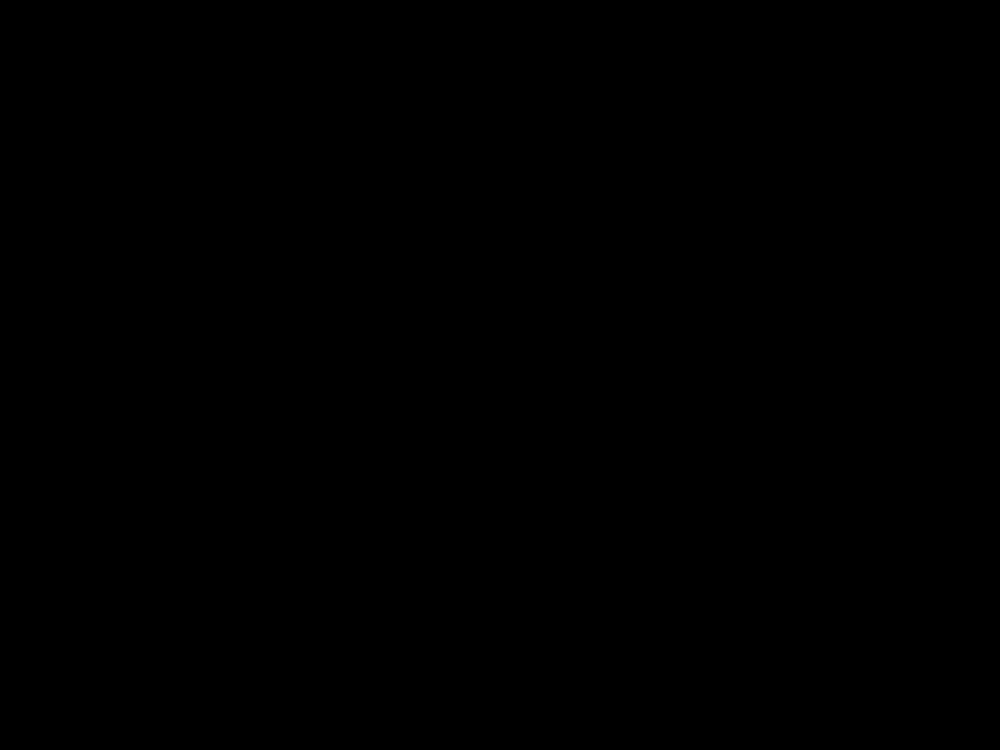
\includegraphics[width=30mm]{images/placeholder.png}}}%
%   \caption{Description}
% \end{figure}

% \begin{figure}[h]
%   \centerline{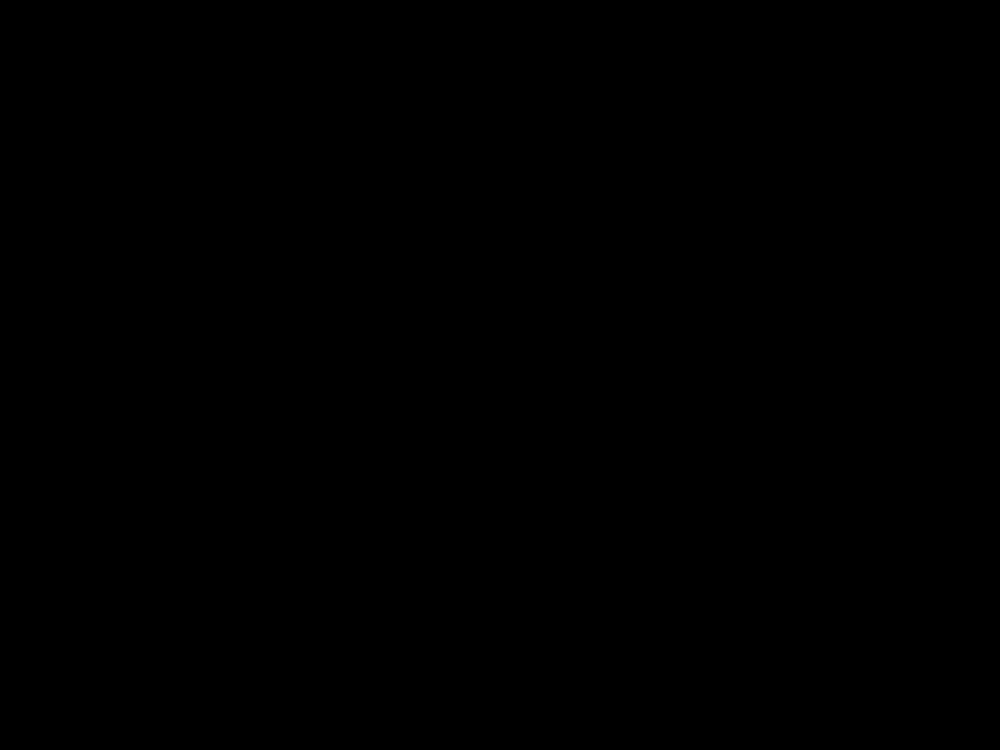
\includegraphics[width=50mm]{images/placeholder.png}}
%   \caption{Description}
% \end{figure}

%Template for a simple table 
%\begin{table}[h]
%   \caption{Description} %title of the table
%   \centering % centering table
%   \begin{tabular}{l rr} % creating three columns
%     \hline\hline %inserting double-line
%     & & \\ [0.5ex] % Insert half line vertical spacing
%     \hline % inserts single-line
%     & & \\ 
%     & & \\
%     & & \\
%     & & \\
%   \hline % inserts single-line
%   \end{tabular}
%   \label{tab:hresult}
% \end{table}
%-----------------------------------------------

\begin{document}


\section{Introduction to Rigid body dynamics}

\subsection{General Workflow}
\begin{figure}[h]
  \centerline{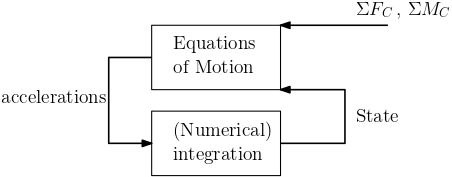
\includegraphics[width=120mm]{images/Dynamics_Work_Flow.png}}
  \caption{The general workflow for solving Dynamics problems}
\end{figure}
Equation's of motion (EOM's) are usually found using Newton's second law of motion ($\vec{F} = m\vec{a}$). There are different ways of derriving EOM's such as using Euler-Lagrange equations or Hamilton-Jacobi equations. In general the work flow of dynamics involves derriving EOM's using those to find accelerations and using (numerical) integration to find the state at a given time $t$.


\subsection{Coordinate systems and triads}
A coordinate system is a set of 3 orthogonal unit vectors with a defined origin. A triad is only defined by the direction of the 3 orthogonal unit vectors. It does not have a defined origin. Both obey the right-hand-rule.
\begin{figure}[h]
  \centering
  \subfloat[A Coordinate system]{{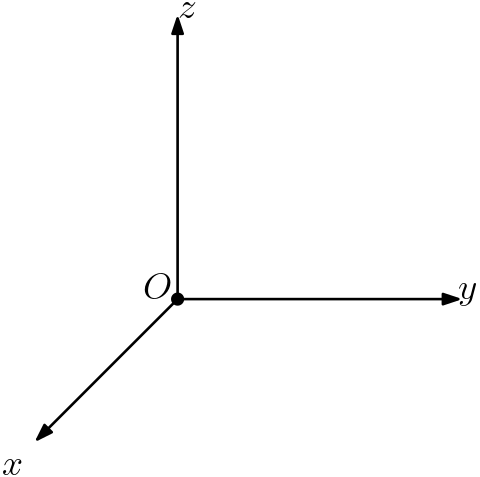
\includegraphics[width=50mm]{images/Coordinates.png}}}%
  \qquad
  \subfloat[A triad]{{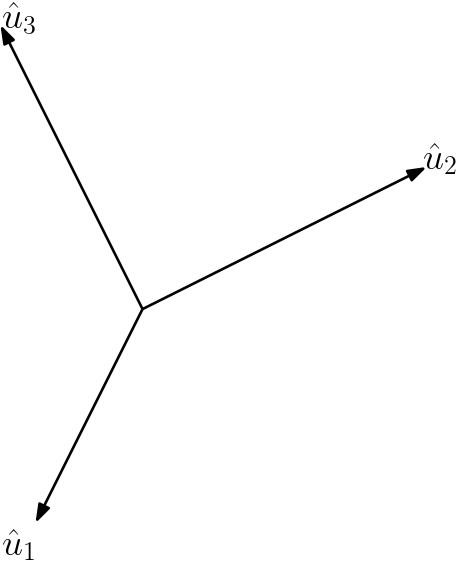
\includegraphics[width=50mm]{images/Triad.png}}}%
  \caption{The difference between a coordinate system and a triad. Note that the triad has no defined origin and only represents 3 directions in space.}
\end{figure}


\subsection{Notation stuff}
A top left superscript is used to denote when the components of the vector are projections of the vector in coordinate direction of the triad. Triad's are denoted by curly math letters:
\begin{equation}
  ^{\mathcal{B}}\vec{q} = \begin{pmatrix} q_{b1}\\ q_{b2}\\ q_{b3}\\ \end{pmatrix}
  \quad \text{or} \quad
  ^{\mathcal{N}}\vec{a} = \begin{pmatrix} a_{n1}\\ a_{n2}\\ a_{n3}\\ \end{pmatrix}
\end{equation}
A bottom right subscript denotes a point in space. For example $\vec{M}_C$ denotes the moment vector about point $C$.
Position vectors are denoted as $\vec{r}_{A/P}$. The slash denotes relative to which point we are considering the position vector. This means that in this case we are considering the vector $\vec{r}$ which goes from some point $P$ randomly oriented in space to some other point $A$, also randomly oriented in space.s
\begin{figure}[h]
  \centerline{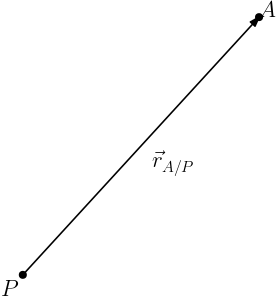
\includegraphics[width=50mm]{images/Position.png}}
  \caption{The position vector $\vec{r}_{A/P}$ visualized.}
\end{figure}


\end{document}